\documentclass[letterpaper,12pt]{article}
\usepackage{tabularx} % extra features for tabular environment
\usepackage{amsmath, amssymb, mathtools}  % improve math presentation
\usepackage{graphicx} % takes care of graphics including machinery
\usepackage{url}
\usepackage{chemfig}
\usepackage[margin=1in,letterpaper]{geometry} % decreases margins
\usepackage{caption}
\usepackage{adjustbox}
\usepackage{cite} % takes care of citations
\usepackage[final]{hyperref} % adds hyperlinks inside the generated pdf file
\hypersetup{
	colorlinks=true,       % false: boxed links; true: colored links
	linkcolor=blue,        % color of internal links
	citecolor=blue,        % color of links to bibliography
	filecolor=magenta,     % color of file links
	urlcolor=blue         
}
\usepackage{blindtext}
\usepackage{amsfonts}
\usepackage{tikz}
\usepackage{standalone}
\usepackage{xcolor}
\usepackage{bookmark}
\usepackage{chemformula}

\setchemfig{atom sep=4em}
\captionsetup{justification=centering}
\definecolor{darkgray}{gray}{0.3}
% \newcommand{\annot}[1]{{\textcolor{darkgray}{\textit{#1}}}}
\newcommand{\annot}[1]{\textcolor{darkgray}{\textit{#1}}}
%++++++++++++++++++++++++++++++++++++++++

\renewcommand{\footnoterule}{%
  \kern-3pt % space above the rule
  \hrule width \textwidth height 0.4pt
  \kern5pt % space below the rule
}

\begin{document}
% TODO: Make the title page centered and in a single page
\title{Gene Regulation \& Epigenetic Processes}
\author{Harsh Agrawal}
\date{\today}
\maketitle

\begin{abstract}
	This notebook compiles content from Molecules Cells and Processes module delivered by Prof.\ Claire Higgins (2nd Year Imperial College London MBE). A total of 6 lectures are covered in these notes. Please suggest any relevant changes/improvements at \href{ha1822@ic.ac.uk}{ha1822@ic.ac.uk}.
\end{abstract}

\tableofcontents
\newpage
\section{Structure and Organization of DNA}
\subsection{Structure of DNA}
We begin our discussion by first establishing the basics of genetics which is the study of genes, and heredity. As we know, genetic information is captured in the form of DNA which is present in all cells of the body.

DNA (or De-oxy Ribonucleic Acid) is a polymer made up of monomeric units which are called nucleotides. Each nucleotide comprises of three parts: a ribose sugar backbone, a nitrogenous base, and three phosphate groups.\ \vspace{.5cm}

\begin{figure}[!h]
	\centering
	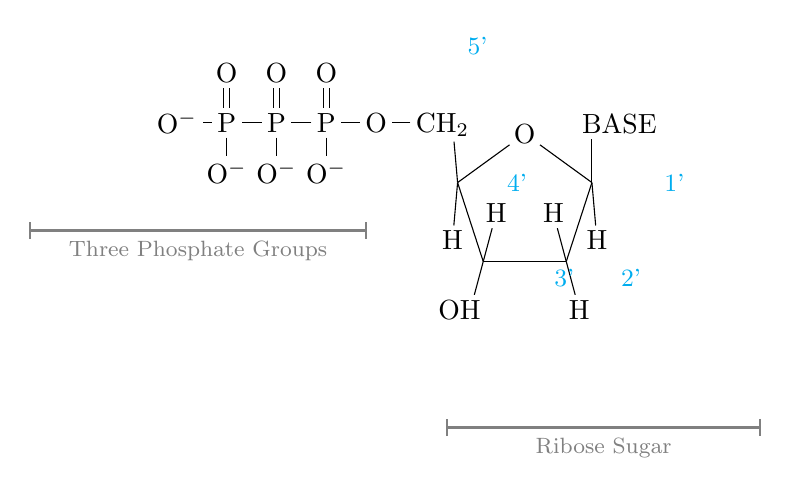
\begin{tikzpicture}
		% \draw[gray!50, dashed, step=1] (-5.9,-3.9) grid (5.9,2.9); % Add this line to draw a grid
		\node[inner sep=0pt] (chemfig)
		{\chemfig{ ([::18]*5((-[:-105, .6] OH)(-[:75, .6]H)-(-[:105, .6] H)(-[:-75, .6] H)-(-[2, .7]BASE)(-[:-85, .7]H)-O-(-[:-95, .7] H)(-[:95, .7] CH_{2}(-[:180, 0.6]O-[:180, 0.6]P(=[90,0.6]O)(-[-90,0.6]O^{-})-[:180, 0.6]P(=[90,0.6]O)(-[-90,0.6]O^{-})-[:180, 0.6]P(=[90,0.6]O)(-[-90,0.6]O^{-})-[:180, 0.6]O^{-}))-)) }};
		\node[below of=chemfig, node distance=3cm, font=\footnotesize]{};

		\draw[|-|, gray, thick] (0.5,-3) -- (4.5,-3) node[midway, below, font=\footnotesize] {Ribose Sugar};

		\draw[|-|, gray, thick] (-4.8,-0.5) -- (-0.5,-0.5) node[midway, below, font=\footnotesize] {Three Phosphate Groups};

		\node[text=cyan, font=\small] at (3.4,0.1){1'};
		\node[text=cyan, font=\small] at (2.85,-1.1){2'};
		\node[text=cyan, font=\small] at (2,-1.1){3'};
		\node[text=cyan, font=\small] at (1.4,0.1){4'};
		\node[text=cyan, font=\small] at (0.9,1.85){5'};
	\end{tikzpicture}
	\caption{Structure of a Nucleotide}
\end{figure}

Some important details to note about the structure of DNA are:
\begin{itemize}
	\item The Carbons in the Ribose sugar are named with the convention of 1' Carbon, 2' Carbon, so on and so forth. The purpose of putting the `prime' after the Carbon number is to particularly specify the Carbon of the sugar ring as opposed to the Carbon of the nitrogenous base (attached at the 5' end).
	\item At the 2'C, there is a Hydrogen atom as apposed to a Hydroxyl group (-OH). This is why DNA is called `De-Oxy' Ribonucleic Acid. In RNA, the 2'C has a Hydroxyl group.
	\item A single nucleotide has three phosphate groups
	      (\ch{PO4^3-}) whereas a nucleotide part of the DNA chain only contains one phosphate group. The other two phosphate groups are lost during the formation of the DNA chain. The negative charge on the Phosphate group gives DNA its overall negative charge.
\end{itemize}

There are four nitrogenous bases (or nucleobases) that are found in DNA and are classified into two groups:
\begin{itemize}
	\item Purines: Adenine and Guanine. Purines have two N-C rings.
	\item Pyrimidines: Cytosine and Thymine. Pyrimidines have only one N-C ring. \textit{Note: In RNA, Thymine is replaced by Uracil.}
\end{itemize}

A nitrogenous base, part of the nucleotide, is referred by its full name which for example, in case of Adenine, would be 2' de-oxyadenosine triphosphate or \textbf{A}. For ease of writing, these nucleotides are often referred to by their first letter shortcodes: A, T, C, and G.

Two nucleotides are covalently linked together by a phosphodiester bond between an Oxygen of Phosphate group  (at 5' C) of one nucleotide and the 3' Carbon of the sugar of the other nucleotide. This forms the sugar-phosphate backbone of the DNA. A DNA sequence is read from the 5' end (free Phosphate group) to the 3' end (free Hydroxyl group).

\begin{figure}[!h]
	\centering
	\begin{tikzpicture}
		% Top DNA
		% \draw[gray!50, dashed, step=1] (-5.9,-3.9) grid (8.9,8); % Add this line to draw a grid
		\node[inner sep=0pt] at (0,5) (chemfig)
		{\chemfig{ ([::18]*5((-[:-105, .6] O)(-[:75, .6]H)-(-[:105, .6] H)(-[:-75, .6] H)-(-[2, .7]BASE)(-[:-85, .7]H)-O-(-[:-95, .7] H)(-[:95, .7] CH_{2}(-[:180, 0.6]O-[:180, 0.6]P(=[90,0.6]O)(-[-90,0.6]O^{-})-[:180, 0.6]O^{-}))-)) }};
		\node[below of=chemfig, node distance=3cm, font=\footnotesize]{};

		% Lower DNA
		\node[inner sep=0pt] at (2.75,-0.2) (chemfig)
		{\chemfig{ ([::18]*5((-[:-105, .6] OH)(-[:75, .6]H)-(-[:105, .6] H)(-[:-75, .6] H)-(-[2, .7]BASE)(-[:-85, .7]H)-O-(-[:-95, .7] H)(-[:95, .7] CH_{2}(-[:180, 0.6]O-[:180, 0.6]P(=[-90,0.6]O)-[:180, 0.6]O^{-}))-)) }};
		\node[below of=chemfig, node distance=3cm, font=\footnotesize]{};

		\draw[-, red, thick] (0.3, 1.9) -- (0.3, 2.4);

		\draw[->, gray, thick] (-1, 2.2) -- (0.05, 2.2) node[xshift=-2.9cm, font=\footnotesize]{Phosphodiester Bond};
	\end{tikzpicture}
	\caption{Formation of a Phosphodiester Bond}
\end{figure}

Nuclebases in the nucleotides also tend to form Hydrogen bonds with an opposing DNA strand. `A' double bonds to `T' whereas `C' triple bonds to `G'. This is called complementary base pairing. The two strands of DNA are anti-parallel to each other, meaning that the 5' end of one strand is opposite to the 3' end of the other strand.

To maximize the efficiency of base-pair packing, the sugar phosphate backbone wind around each other to give DNA a helical structure. In this structure, the non-polar bases occupy the interior whereas the negatively charged phosphate group occupy the exterior. This gives DNA its famous double helix structure. The length of the DNA is referred by base-pairs (bps). The human genome has around 3 billion base pairs.

\subsection{Chromosomes and Organization of DNA}

\begin{figure}[h!]
	\centering
	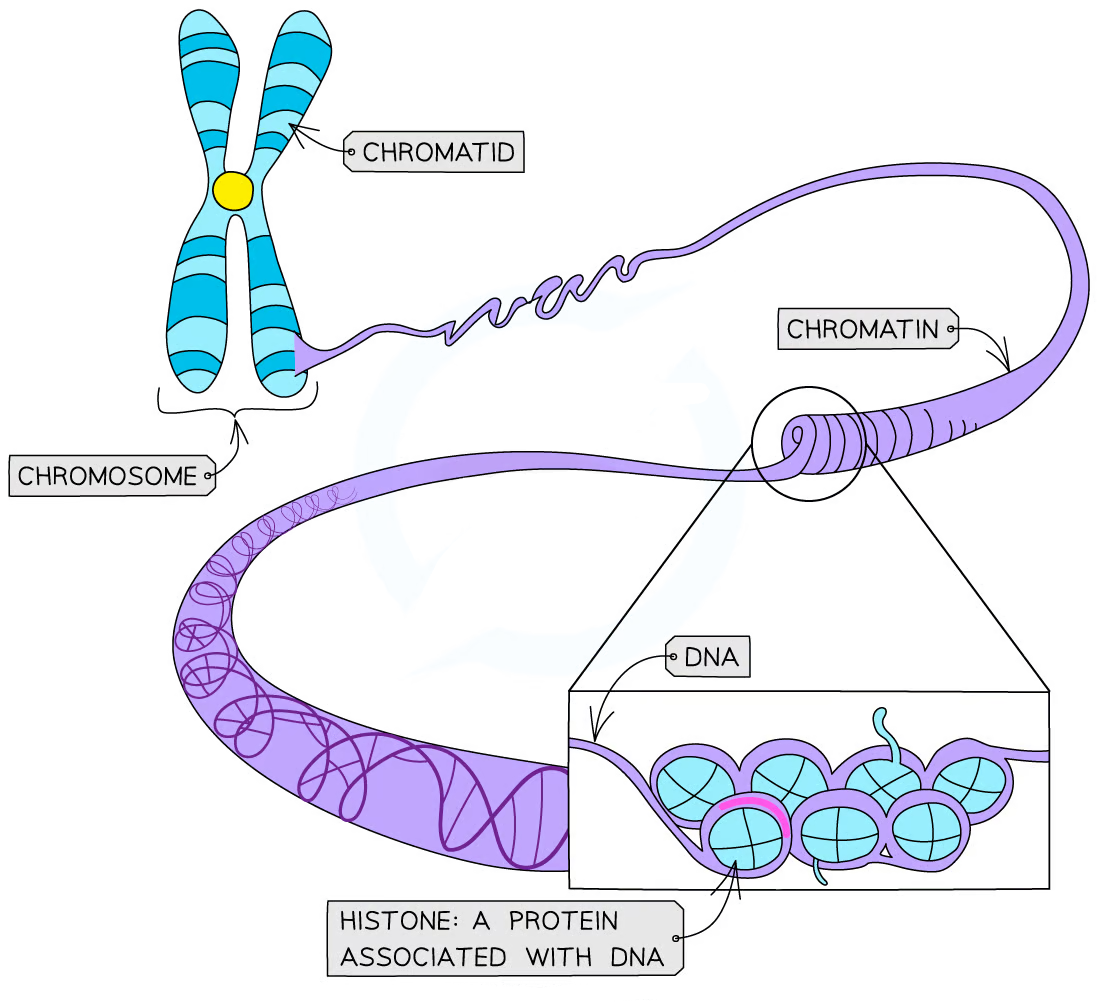
\includegraphics[width=0.6\textwidth]{figures/chromosomes_unraveled.png}
	\caption{Compression of DNA into Chromosomes. Taken from \url{https://www.savemyexams.com/a-level/biology/cie/22/revision-notes/}}\label{fig1}
\end{figure}

DNA is present in a compressed form in the nucleus of the cell called chromosomes.
\begin{itemize}
	\item Around 146 Base Pairs of DNA winds around 8 `Histone' proteins to form a \textbf{nucleosome}. This is the basic unit of DNA packaging. The positive charge on Histones and the negative charge on DNA facilitates their binding. These nucleosomes are often referred as `beads on a string' (DNA=string, Histones=beads).
	\item Nucleosomes pack into a coil called \textbf{chromatin} (or chromatin fibres). These chromatin fibres further coil into loops and form a \textbf{chromatid}. In a somatic cell, there are 46 chromatids. The above image shows two chromatids forming a \textbf{chromosome}.
	\item A chromosome can have one or two chromatids (called sister chromatids). In the growth phase, each chromosome in a somatic cell contains one chromatid but while cell division, each chromatid makes another copy and thus there are 96 chromatids (albiet only 46 chromosomes) in the cell.
\end{itemize}

\begin{figure}[h!]
	\centering
	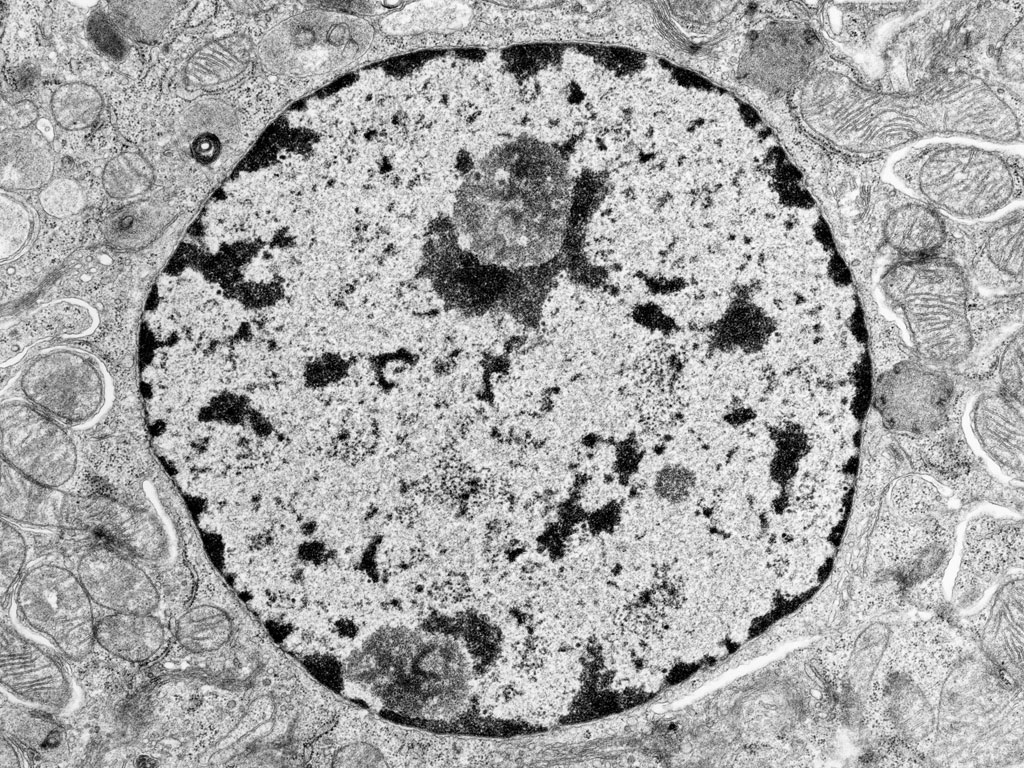
\includegraphics[width=0.6\textwidth]{figures/euchromatin_vs_heterochromatin.jpg}
	\caption{Figure showing euchromatin and heterochromatin. Taken from \url{https://medcell.org/histology/cell_lab/euchromatin_and_heterochromatin.php}. The dark regions are heterochromatin whereas the lighter region are euchromatin}\label{fig2}
\end{figure}

De-condensed chromatin is found within the nucleus in tightly packed regions called \textbf{Heterochromatin} and loosely packed regions called \textbf{Euchromatin}. This can be observed in Figure~\ref{fig2}. Euchromatin is more abundant (92\%) than heterochromatin (8\%)Euchromatin is transcriptionally active.

\subsection{Epigenetic Modifications on Histones \& DNA}

A Nucleosome is formed by wrapping of DNA around a histone octamer. Two copies of 4 different histone proteins (H2A, H2B, H3, H4) form this octamer. Approximately 146 base pairs of DNA wrap around the octamer. The DNA that links two nucleosomes is called \textbf{linker DNA} and is around 20 base pairs long.

\begin{figure}[!h]
	\centering
	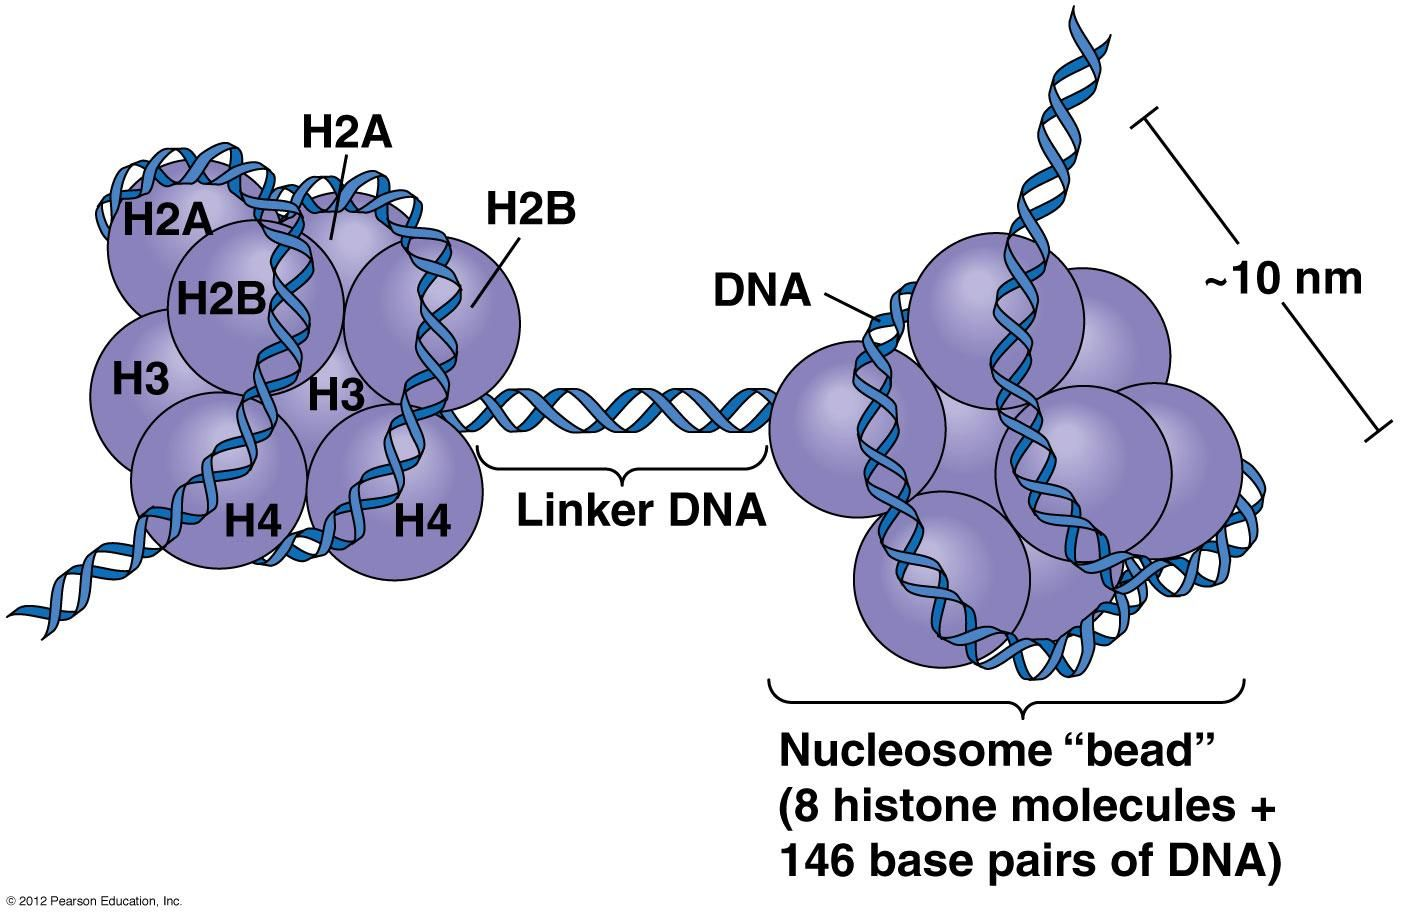
\includegraphics[width=0.6\textwidth]{figures/histones.jpeg}
	\caption{Figure showing DNA wrapped around histones. Taken from \url{https://www.extremetech.com/extreme/213582-new-findings-shed-light-on-fundamental-process-of-dna-repair}.}\label{fig3}
\end{figure}

The size of DNA wrapped around the histone octamer was found via MNAse digest enzyme tests which were used to digest the linker DNA and keep the wrapped DNA uncleaved. This DNA was then run on a gel to obtain the size of the DNA. The original structure estimate of nucleosomes (`beads on a string') was obtained by an electron micrograph.\vspace{1em}

Histones play a crucial role in gene expression as modifications to histones have the ability to make the DNA more active, or repressed for transcription, as well as affect chromosomal packing. These changes include: methylation (most common), phosphorylation, acetylation, ubiquitination, and sumoylation.

\paragraph{Acetylation of Histones}\mbox{}\\
\begin{figure}[!h]
	\centering
	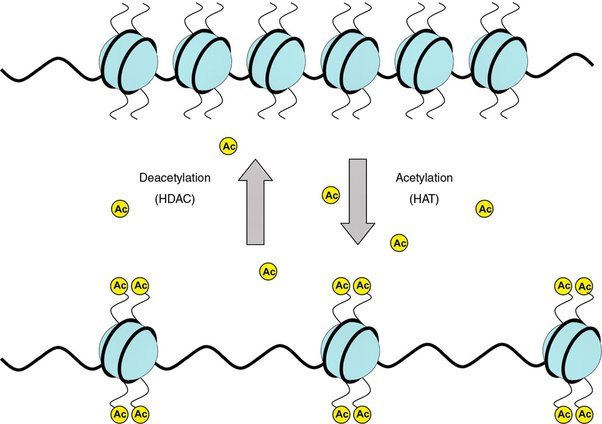
\includegraphics[width=0.8\textwidth]{figures/histone_acetylation.jpeg}
	\caption{Histone Acetylation. Taken from Eslaminejad, Mohamadreza \& Fani, Nesa \& Shahhoseini, Maryam. (2013)}\label{fig4}
\end{figure}

One of the most common ways to modify histones is by acetylation. The process occurs as follows:
\begin{itemize}
	\item The Enzyme group \textbf{Histone Acetyl Transferases (HATs)} transfer the acetyle group from acetyl CoA to the lysine side-chain of the histone protein which reduces the overall positive charge on the histone\cite{Bannister_Kouzarides_2011}.
	\item This reduction of positive charge weakens the interaction between the histone and the DNA (as DNA is negatively charged), making the DNA more unwound and therefore more accessible for transcription.
	\item This relaxed chromatin can be reversed back to tightly wound chromatin by another class of enzymes called \textbf{Histone Deacetylase (HDAC)} which remove the acetyl group to bring back the original positive charge on the histones.
\end{itemize}

Mutations in genes correlated to HDAC have been known to cause cancer as it impacts chromosomal packing. This is why HDAC inhibitors are also being explored as a potential cancer treatment.

\paragraph{Methylation of Histones}\mbox{}\\
Methylation is another method of modifying histones.
\begin{itemize}
	\item The enzyme group responsible for methylation is \textbf{Histone Methyl Transferases (HMTs)} which adds a methyl group to the histone protein whereas the enzyme group \textbf{Histone Demethylases (HDMs)} are responsible for removing the methyl group.
	\item There are different methylation marks that are named as `H3K27me3', `H3K20me3', etc.
	      \begin{itemize}
		      \item `H3' refers to the third histone protein.
		      \item `K' refers to the lysine residue.
		      \item `20' refers to the position of the lysine residue in the histone protein.
		      \item `me3' refers to the addition of three methyl groups on the lysine residue\footnote{Amino Acids as part of proteins are also called \textit{residues}.}. There can be one, two, or three methyl groups added per lysine residue.
	      \end{itemize}
	\item Some of these marks are repressive while some are activating (can differ from cell to cell).
\end{itemize}

\paragraph{Methylation of DNA}\mbox{}\\
\begin{figure}[!h]
	\centering
	\begin{tikzpicture}

		\node[text=cyan, font=\small] at (10.5,1.2){5'};
		\node[text=cyan, font=\small] at (2.8,1.2){5'};

		\setchemfig{scheme debug=false, arrow coeff=1.5}
		\setchemfig{atom sep=35pt}
		\begin{scope}
			\schemestart
			\chemfig{C*6((=0)-N(-H)-CH=C(-H)-C(-NH_3)=N-)}\arrow{->[DNMT][SAM]}
			\chemfig{C*6((=0)-N(-H)-CH=C(-CH_3)-C(-NH_3)=N-)}
			\schemestop
		\end{scope}
	\end{tikzpicture}
	\caption{Methylation of Lysine Residue}\label{fig:lysine_methylation}
\end{figure}

Apart from occuring on histones, methylation can also occur in DNA by the addition of a methyl group to the 5th Carbon of the \textbf{Cytosine} base (only) on the DNA strand (figure~\ref{fig:lysine_methylation}). This is catalyzed by a class of enzymes called \textbf{DNA Methyl Transferases (DNMTs)}. DNMTs transfer a methyl group from S-adenosyl methionine (SAM) to the cytosine base. This only occurs on a Cytosine base adjacent to a Guanine base, also referred to as a \textbf{CpG} site\footnote{CpG stands for Cytosine-Phosphate-Guanine.}; eg: TAT\textbf{C}GTGCT (\textit{only the bold C can be methylated}).

DNA methylation is a repressive mark and it makes the DNA more packed and less accessible for transcription. Thus, there is an increase in DNA methylation in heterochromatin as compared to euchromatin.


\subsection{Gene Regulation due to Epigenetic Modifications}
Gene expression is highly regulated by these epigenetic changes. When the chromatin is in a repressed state (methylated), the DNA is inaccessible for the transcription factors to bind to the promotor regions of the respective genes, thus hindering the expression of the gene.

\begin{figure}[!h]
	\centering
	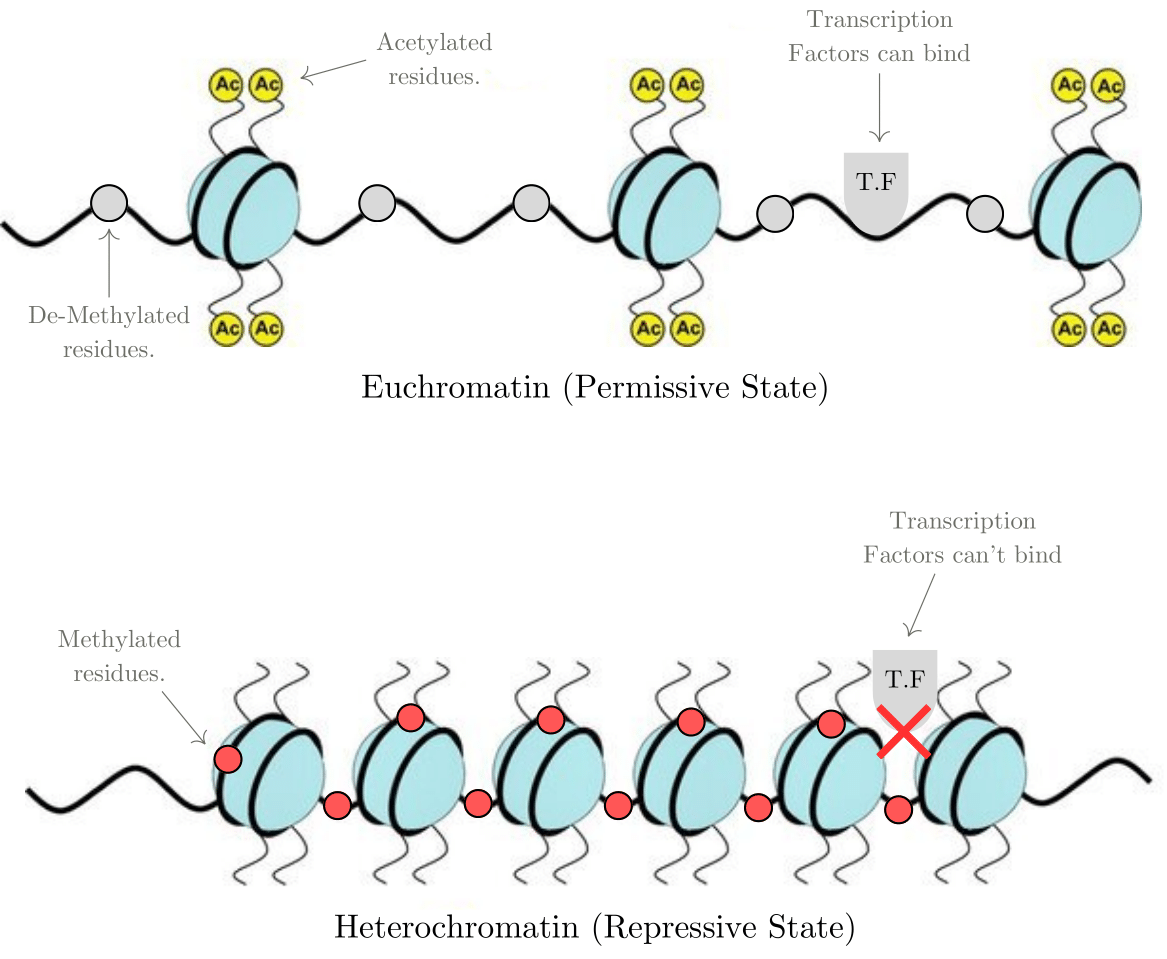
\includegraphics[width=0.8\textwidth]{figures/transcription_factors.png}
	\caption{Annotations showing how repressed chromain is inaccessible for transcription factors to bind. Source image taken from Eslaminejad, Mohamadreza \& Fani, Nesa \& Shahhoseini, Maryam. (2013)}\label{fig:transcription_factors}
\end{figure}

Environmental factors play an important role in epigenetic modifications to chromatin. For example, a study conducted in plants revealed that cold stress (an environmental factor) resulted in the degredation of Histone Deacetylase (HDAC), which in turn increased acetylation, and increase transcription\cite{Park_Lim_2018}.\vspace{1.5cm}

The transcriptional state of chromatin can be more presicely stated as:
\begin{itemize}
	\item \textbf{Active Chromatin}: Active chromatin is accessible for transcription factors to bind and the genes can thus be transcribed.
	\item \textbf{Posed Chromatin}: In the poised state, the chromatin is physically closed and the majority of the transcription factors can't physically bind. However, its found that a set of transcription factors, called the the \textbf{pioneer factors}, can bind to this poised state. These pioneer factors can then recruit enzymes such as HATs etc. to acetylate and open up the chromatin for transcription.
	\item \textbf{Repressed Chromatin}: In the repressed state, the chromatin is tightly packed and none of the transcription factors (including pioneer factors) can bind to the promotor regions of the genes.
\end{itemize}

Histone marks distinguish between repressed and permissive states. For example, the presence of a trivalent motif: H3K4me1, H3K27ac, and H3K9me3 on the chromatin makes it permissive whereas it's absence makes the chromatin repressive.\vspace{0.5cm}

\setlength{\fboxsep}{10pt}
\noindent\fbox{%
	\parbox{\textwidth}{%
		\begin{center}
			\textbf{Direct Reprogramming of Fibroblasts}
		\end{center}
		\begin{itemize}
			\item Direct Reprogramming is carried out by adding a few essential transcription factors to Fibroblasts that then swtich on multiple hundreds or more genes required for the fibroblast to be converted to a Neuron.
			\item One such transcription factor is \textbf{Ascl1} which when added to the fibroblasts is able to convert them into neurons, whereas when the same transcription factor is added to Keratinocytes, conversion to neurons isn't observed.
			\item This is because Fibroblasts have permissive chromatin (presence of \textbf{the trivalent motif}) at the Ascl1 binding sites allowing transcription of Ascl1 and all further genes, to occur. The absence of the trivalent motif in the Ascl1 binding regions of Keratinocytes prevent downstream transcription and thus the conversion to Neurons isn't observed.
		\end{itemize}
	}%
}

\newpage
\section{RNA Transcription}
\subsection{Transcription process}
The transcription of gene (DNA $\rightarrow$ RNA) is carried out in three stages: initiation, elongation, and termination.
\begin{figure}[!h]
	\centering
	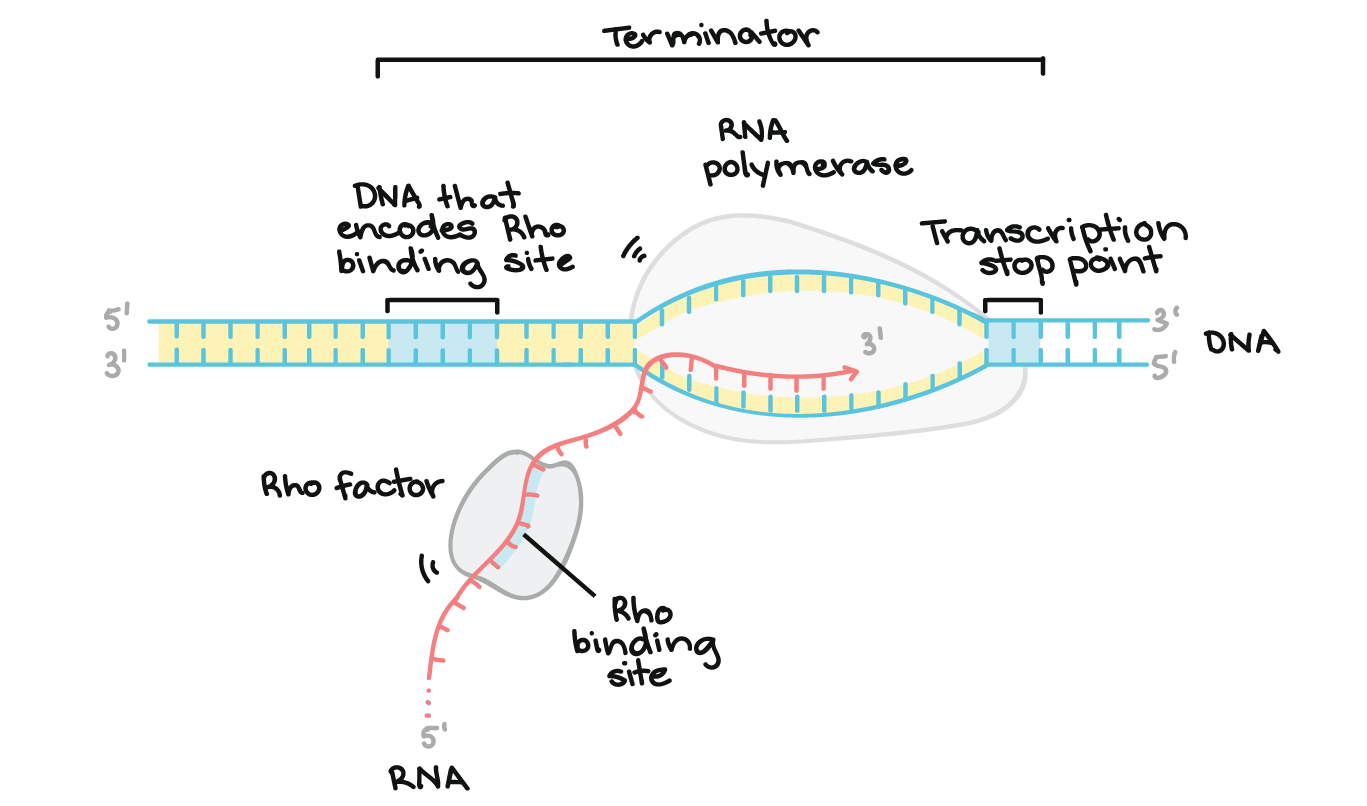
\includegraphics[width=0.8\textwidth]{figures/transc_new.png}
	\caption{Image showing transcription. Source: \url{https://www.khanacademy.org/science/biology/gene-expression-central-dogma/transcription-of-dna-into-rna/a/eukaryotic-pre-mrna-processing}}\label{fig:transcription}
\end{figure}
\subsubsection*{Initiation}
\begin{figure}[!h]
	\centering
	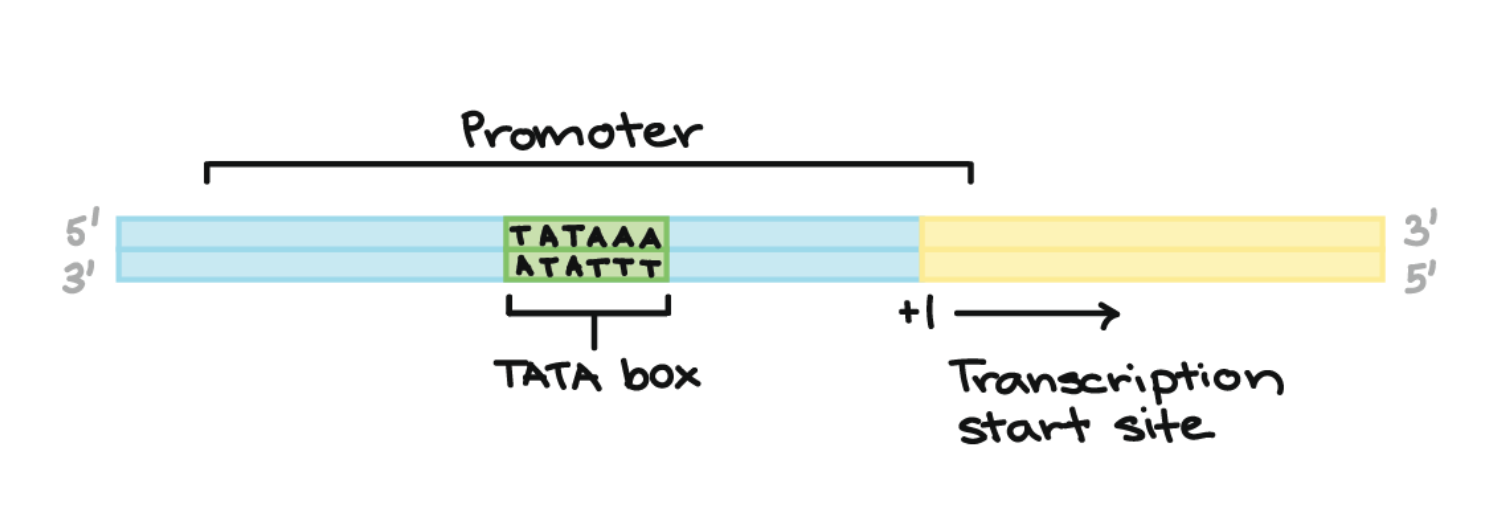
\includegraphics[width=0.8\textwidth]{figures/recognition_site.png}
	\caption{Image showing the TATA Box. Source: \url{https://www.khanacademy.org/science/biology/gene-expression-central-dogma/transcription-of-dna-into-rna/a/eukaryotic-pre-mrna-processing}}\label{fig:TATABOX}
\end{figure}
\begin{itemize}
	\item The enzyme responsible for the conversion of DNA to RNA is called \textbf{RNA Polymerase}. binds to a region of the DNA (in the 5' end) called the \textbf{promotor region}. The promotor region is a sequence of DNA that signals the start of the gene.
	\item The site on the DNA from which the first RNA nucleotide is transcribed is called the +1 site, or the \textbf{initiation site}. Nucleotides that come before the initiation site are given negative numbers and said to be upstream. Nucleotides that come after the initiation site are marked with positive numbers and said to be downstream\footnote{Sentence taken directly from: https://www.khanacademy.org/science/biology/gene-expression-central-dogma/transcription-of-dna-into-rna/a/stages-of-transcription}.
	\item In eukaryotes, this promoter sequence consists of a region called the \textbf{TATA box} (figure~\ref{fig:TATABOX}) which consists of A, T repeats\footnote{Identified in 1978 and is found in $\sim$30\% of human gene promoters} and is found 25bp upstream of the transcription site.
	      The TATA box is recognized by \textbf{TATA binding protein} (TBP) that is essential to forming the preinitiation complex which then recruits the RNA polymerase to attach and start transcription.
	\item In Cancer, the TATA box is often found to be mutated. In case of Tumor Suppressor Genes, the TATA box is mutated for reduced TBP binding $\longrightarrow$ reduced transcription of Tumor Suppressor Genes $\longrightarrow$ decreased suppression of cancer cells $\longrightarrow$ higher cancer malignancy. In case of Oncogenes, the TATA box might be mutated to increase TBP binding thus promoting the transcription of the oncogenes.
	\item The DNA strand that runs from 5' $\rightarrow$ 3' is called the \textbf{coding strand} or the \textbf{sense} strand. This strand isn't used for transcription. The antiparallel strand (that runs from 3' $\rightarrow$ 5') is called the \textbf{template strand} or the \textbf{anti-sense strand} and is used for transcription.
\end{itemize}

\subsubsection*{Elongation, Termination, and Post-Processing}
\begin{figure}[!h]
	\centering
	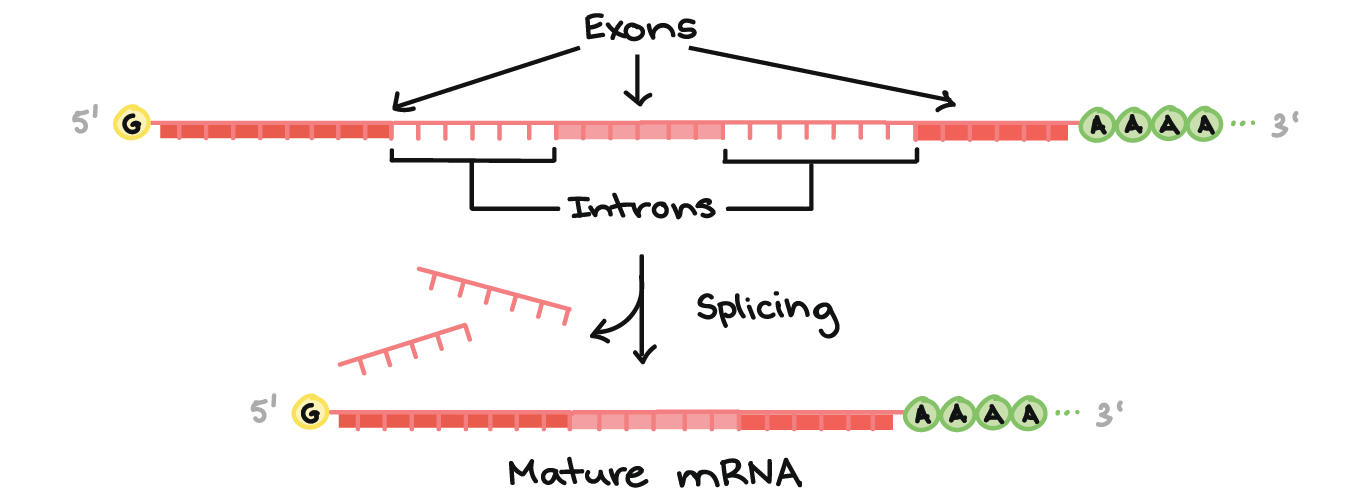
\includegraphics[width=0.8\textwidth]{figures/splicing.png}
	\caption{Image showing Splicing of RNA transcript to mRNA. Source: \url{https://www.khanacademy.org/science/biology/gene-expression-central-dogma/transcription-of-dna-into-rna/a/eukaryotic-pre-mrna-processing}}\label{fig:splicing}
\end{figure}
\begin{figure}[!h]
	\centering
	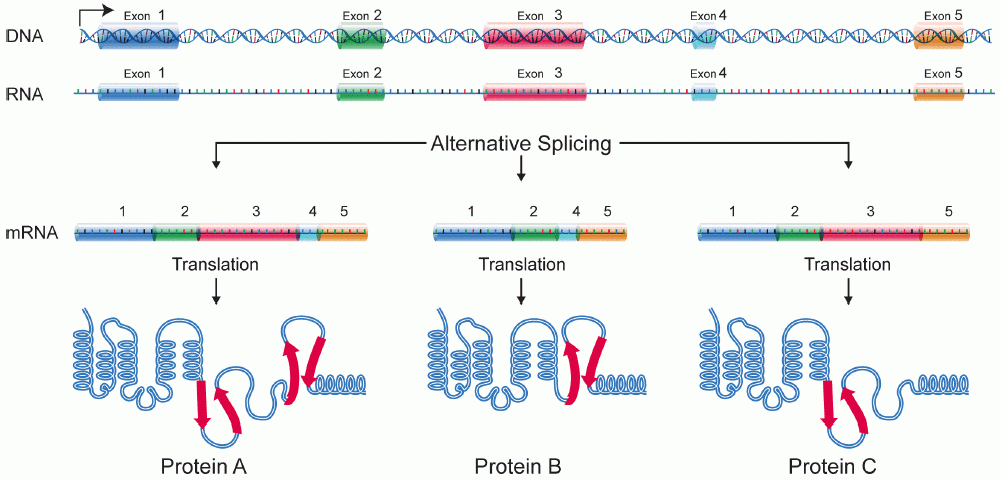
\includegraphics[width=0.8\textwidth]{figures/alternative_splicing.png}
	\caption{Image showing Alternative Splicing to create different mature mRNA transcripts. Source: \url{https://www.khanacademy.org/science/biology/gene-expression-central-dogma/transcription-of-dna-into-rna/a/eukaryotic-pre-mrna-processing}}\label{fig:alternative_splicing}
\end{figure}
\begin{itemize}
	\item The process of Elongation is the extension of the newly synthesized RNA strand. The RNA polymerase moves along the DNA template strand and adds nucleotides to the 3' end of the RNA strand. The RNA polymerase, unlike DNA polymerase, doesn't require a primer to start the elongation process.
	\item The synthesized RNA strand is complementary to the anti-sense strand is thus identical to the sense strand (except for the Uracil base switch in place of Thymine).
	\item This RNA transcript is then processed by the following the addition of a 5' cap and a 3' poly-A tail. This is added to prevent RNA from being degraded.
	\item It's followed by splicing the RNA to remove introns and join exons to form the mature mRNA (figure~\ref{fig:splicing}). Every 5' splice site on an intron usually starts `GT' whereas the 3' splice site ends with `AG'.
	\item The region of the transcript that codes for the protein is called the \textbf{Open Reading Frame (ORF)}. The rest of the transcript is called the \textbf{Untranslated Region (UTRs)}\footnote{Start codon of the ORF is usually `ATG' whereas the stop codon is usually `TAA' / `TAG'.}.
	\item Initially, it was presumed that humans had $sim$ 100,000 genes. However, it was later found that humans only have 20,000 but the number of proteins coded by these genes is 100,000. This was found to be due to \textbf{Alternative Splicing} (figure~\ref{fig:alternative_splicing}) where different exons are joined together to form different mature mRNA transcripts.
	\item It's estimated that $sim 60\%$ of the genes in the human genome have multiple splice variants, thus coding for slightly different proteins.
\end{itemize}
\begin{itemize}
	\item \textbf{5' Promoter Region}: This is the region where relevant proteins such as RNA polymerase and transcription factors bind to initiate transcription of that gene.
	\item \textbf{3' Poly-A Tail}: This is a sequence of Adenine bases added to the 3' end of the RNA transcript. This is important for the stability of the RNA transcript.
	\item \textbf{Protein Coding Region}: This is the region that comprises of \textbf{introns} and \textbf{exons}. Introns are spliced away and exons are joined together to form the mature mRNA that is translated into a protein\footnote{Whole genome sequencing is quite expensive and in-efficient. Since only the exome codes for proteins, whole exome sequening has proven to be a much more efficient alternative}.
\end{itemize}

Introns comprise of over 99\% of the entire genome (not translated to proteins). However, around 90\% of observed phenotype-related mutations are found in exons.

\newpage
\bibliographystyle{plain}
\bibliography{main}
\end{document}
